\documentclass[a4paper,openany]{uantwerpenassignment}

\usepackage[dutch]{babel}
\usepackage{titlesec}
\usepackage{tikz}
\usepackage{pythonhighlight}
\usepackage{amsmath}
\usepackage{array}
\usepackage{subcaption}
\usepackage{listings}\usepackage[nottoc,numbib]{tocbibind}

\renewcommand{\lstlistingname}{Code}

\newenvironment{conditions}
  {\par\vspace{\abovedisplayskip}\noindent\begin{tabular}{>{$}l<{$} @{${}={}$} l}}
  {\end{tabular}\par\vspace{\belowdisplayskip}}

\definecolor{code}{HTML}{ecf0f1}
\definecolor{codetext}{HTML}{d9534f}
\newcommand{\codeword}[1]{
    \colorbox{code}{\texttt{\textcolor{codetext}{#1}}}
}

\newcommand{\reference}[1]{\textit{\ref{#1}. \nameref{#1}}}
\newcommand{\figref}[1]{\textit{Figuur \ref{#1}}}
\newcommand{\coderef}[1]{\textit{Code \ref{#1}}}
\newcommand{\ts}{\textsuperscript}
\newcommand\scalemath[2]{\scalebox{#1}{\mbox{\ensuremath{\displaystyle #2}}}}

\facultyacronym{TI}

\title{\sffamily Chess AI-Agent}
\subtitle{\sffamily5-Artificiële Intelligentie}
\author{\sffamily Mathias Maes, Tijs Van Alphen \\en Willem Van der Elst}

\programme{BA}{IW}{EI}

\academicyear{2020-2021}

\publisher{}

\titleformat{\chapter}{\sffamily\huge\bfseries}{\thechapter.}{10pt}{\sffamily\huge\bfseries}
\titleformat{\section}{\sffamily\LARGE\bfseries}{\thesection.}{10pt}{\sffamily\LARGE\bfseries}
\titleformat{\subsection}{\sffamily\Large\bfseries}{\thesubsection.}{10pt}{\sffamily\Large\bfseries}
\titleformat{\subsubsection}{}{}{10pt}{\sffamily\large\bfseries}


\begin{document}

\sffamily
\maketitle

\tableofcontents

\chapter{Keuze}
\label{keuze}

Het type AI was een belangrijke keuze van dit project. Het moest haalbaar zijn om te implementeren binnen de beperkte tijdsperiode en we moesten onze eigen niet-supercomputers gebruiken om te treinen. Een lijst  met de voor- en nadelen van de verschillende opties werd opgesteld.\\[2 \baselineskip]


\textbf{Search}:\\
Er zijn te veel mogelijke states ($\approx10^{120}$) om de hele tree uit te werken. 

\textbf{Multi-Agent search} (Minimax, Alpha-Beta pruning):\\
Deze methode wordt gebruikt door meerdere bronnen, maar we hebben er nog geen ervaring mee. 

\textbf{Reinforcement learning} (Generalised Q learning):\\
We hebben dit al gebruikt en daarom begrijpen we het al en kunnen we het snel implementeren.\\
Eenmaal getraind, zal het optimaal functioneren. De training heeft echter veel tijd nodig en de keuze van de features is niet zo voor de hand liggend.

\textbf{Neural network/ Deep learning:}
Onze ervaring met Deep learning is nogal beperkt. We weten niet goed wat we als in- en output moeten nemen. \\[2 \baselineskip]


Q-Learning leek ons het interessantst, maar Minimax is haalbaarder en zou sowieso een goed resultaat leveren. Uiteindelijk besloten we om beide methodes uit te werken. We hadden namelijk een thesis\cite{rl} gevonden die een minimax agent gebruikte als feature voor een generalized Q-Learner.

\chapter{Alpha-Beta Pruning}

\section{Utility}
\label{utility}

Onze utility is grotendeels gebaseerd op de rewards van onze Q-Learner die later in dit verslag behandelt worden.
Op dit moment volstaat het om een simpele versie van onze utility te aanschouwen:


$$
u(S) = 
\begin{cases}
 100 &\mbox{Schaakmat gewonnen}\\
    -30 &\mbox{Gelijkspel of Stalemate}\\
    -100 &\mbox{Schaakmat verloren}\\
    c + C + \Delta M + \Delta m + s + f_q &\mbox{Bij overige situaties}
\end{cases}
$$

\begin{conditions}
    c & Of er gecastled is met de vorige move\\
    C & Of het bord in schaak staat\\
    \Delta M & Het materiaal verschil op het bord\\
    \Delta m & Het verschil in mobility\\
    s & De positie score voor alle eigen stukken\\
    f_q & Een gewogen(geleerd of niet-geleerd) aantal features
\end{conditions}

Deze kleine sub-functies worden later nog besproken in \reference{features}.

\chapter{Q-Learning Agent}

\section{Generalization}

De eerste agent die we maakten, was de Q-agent. Deze is generalized omdat, zoals besproken in \reference{keuze}, het praktisch onmogelijk is om elke staat te bezoeken. Daarom dat we niet 'gewoon' Q-learning kunnen gebruiken, maar wel generalized Q-learning.

\section{Features}
\label{features}

We hebben een hoop features gedefinieerd. Deze zijn voornamelijk gebaseerd op features uit de paper\cite{rl}. De bedoeling van deze features is om een state zo goed mogelijk te definiëren. Je kan hieronder een beschrijving vinden van elks van onze 55 features.

We berekenen onze features met deze formule:

$$
Q(s,a) = \sum_{i} w_{i} \cdot \sigma \left( f_i(s, a)\right)
$$

De $\sigma(x)$ die we in de berekening zien wordt als volgt gedefinieerd:

$$
\sigma^*(x) = \frac{2}{1 + e^{-x}} - 1
$$

Dit is een aangepaste versie van de bekende sigmoid\cite{WSF} functie. Onze versie zorgt in tegenstelling tot de originele er voor dat waardes in het interval $\left]-1,1\right[$ vallen.\\
Hier zie je de grafiek van de functie:

\begin{figure}[h]
    \centering
    \begin{tikzpicture}[scale=2]
        \draw[->] (-2, 0) -- (2, 0) node[right] {$x$};
        \draw[->] (0, -1.2) -- (0, 1.2) node[above] {$y$};

        \draw[dashed] (-2, 0.5) -- (2, 0.5);
        \node (A) at (-2, 0.6) {\tiny $1$};

        \draw[dashed] (-2, -0.5) -- (2, -0.5);
        \node (B) at (-2, -0.6) {\tiny $-1$};

        \draw[scale=0.5, domain=-3.9:3.9, smooth, variable=\x, blue] plot ({\x}, { 2/(1 + exp(-\x)) - 1 });
        \node[blue] (C) at (0.4, 0.32) {$\sigma^*$};
    \end{tikzpicture}
    \caption{$\sigma^*(x)$} \label{fig:sigmoid}
\end{figure}



\subsection{Amount of Pieces}
De meest voor de hand liggende feature die we gebruiken, is het aantal stukken per type op een bord. We berekenen dit aantal voor zowel de onze als die van de tegenspeler. Elk type krijgt dus 2 features.

Op deze manier zal onze Q-agent leren dat het voordelig is om het aantal stukken van zichzelf hoog te houden en die van de opponent laag te houden.

Het laatste wat we ook nakijken is de feature \codeword{AmountBalancePieces()} deze zal de material value van alle stukken van de speler berekenen en de material value van de tegenspeler er af trekken. Wanneer dit getal negatief is, betekent dat dus dat de opponent er op dit vlak beter voor staat.


\subsubsection{Material value}
Elk soort schaakstuk krijgt een cijfer dat zijn waarde bepaalt. Zo krijgt de koningin een hogere waarde dan een pion, omdat de koningin belangrijker is. In \coderef{code:material} staat de implementatie van hoe de schaakstukken zich verhouden t.o.v. elkaar.

\begin{lstlisting}[style=mypython,caption={Material Function},captionpos=b,label={code:material}]
def getMaterialValue(piece_type):
    if piece_type is chess.PAWN:
        return 1
    elif piece_type is chess.KNIGHT or piece_type is chess.BISHOP:
        return 3
    elif piece_type is chess.ROOK:
        return 5
    elif piece_type is chess.QUEEN:
        return 9
    elif piece_type is chess.KING:
        return 10

    return 0
\end{lstlisting}

\subsection{Checkmate}

De feature \codeword{Checkmate()} gaat kijken of we bij de volgende actie de opponent schaakmat kunnen zetten.

\subsection{Next Checkmate}

In deze feature gaan we kijken of de volgende zet van de tegenspeler kan zorgen dat wij schaakmat worden gezet.

\subsection{Mobility}
De \codeword{Mobility.py} file berekent voor elke type schaakstuk hoeveel vakjes het stuk kan bereiken. 

Dit wordt gebruikt voor de mobility features. Hierbij gaan we voor elke type schaakstuk kijken op hoeveel vakjes die kan terechtkomen. Dit zullen we ook weer doen voor zowel de speler als de tegenspeler.

De feature \codeword{MobilityRookS()} zal voor elke Rook (toren) van de eigen speler (S in de functie staat voor self) berekenen op hoeveel vakjes die kan komen en bij elkaar optellen.

Voor het berekenen van de legal moves gebruikte we de functie \codeword{islegal(Move)} op het huidige bord.  Hier hebben we wat problemen mee ondervonden voor de opponent omdat we enkel stukken kunnen verplaatsten van diegene die aan beurt is. Alle moves van de opponent zijn dus illegal. Onze oplossing hiervoor is om een copy van het bord maken gevolgd door een board turn, op deze manier speel je dan zogezegd even als de opponent op het gekopieerde bord. 


\subsection{Attackers}
Deze attacked features laten weten hoeveel van de schaakstukken van een bepaald type aangevallen kunnen worden door de opponent met inferieure schaakstukken. 

Zo zal bijvoorbeeld de \codeword{AttackedRooksS()} feature calculeren hoeveel van zijn torens kunnen worden aangevallen door een pion, een paard of een loper van het andere team.

Voor de opponent versie van deze features te berekenen hebben we het probleem op dezelfde manier opgelost als bij moblility .

\subsection{Forks}

De volgende twee features zijn zowel voor de speler als de tegenspeler geïmplementeerd.

\subsubsection{Pawn Fork}
Pawn fork gaat kijken hoeveel pionnen 2 superieure stukken van de tegenstander aanvalt.

In \figref{fig:pawnFork} zal pion op d4 meetellen bij de pawn fork som, omdat deze 2 schaakstukken met een hogere material value kan nemen. Terwijl pion op g4 niet zal worden meegeteld.

\subsubsection{Knight Fork}
Gelijkend aan de Pawn fork zal de Knight fork ook kijken hoeveel paarden 2 superieure schaakstukken van de tegenspeler kan nemen.

In \figref{fig:knightFork} zal het paard op d5 worden meegeteld, maar het paard op g2 niet. Het paard op g2 wordt niet meegeteld omdat het paard dat deze kan nemen niet superieur is t.o.v. zichzelf.


\begin{figure}[h]
    \centering
    \begin{subfigure}{.4\textwidth}
        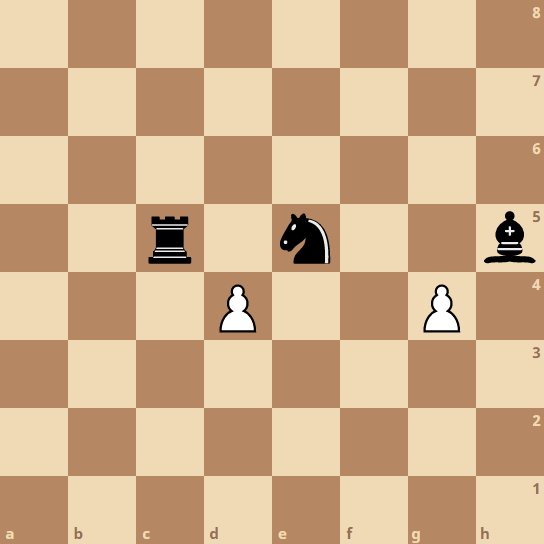
\includegraphics[width=170pt]{images/pawnFork.png}
        \caption{Example of pawn fork}
        \label{fig:pawnFork}
    \end{subfigure}
    \begin{subfigure}{.4\textwidth}
        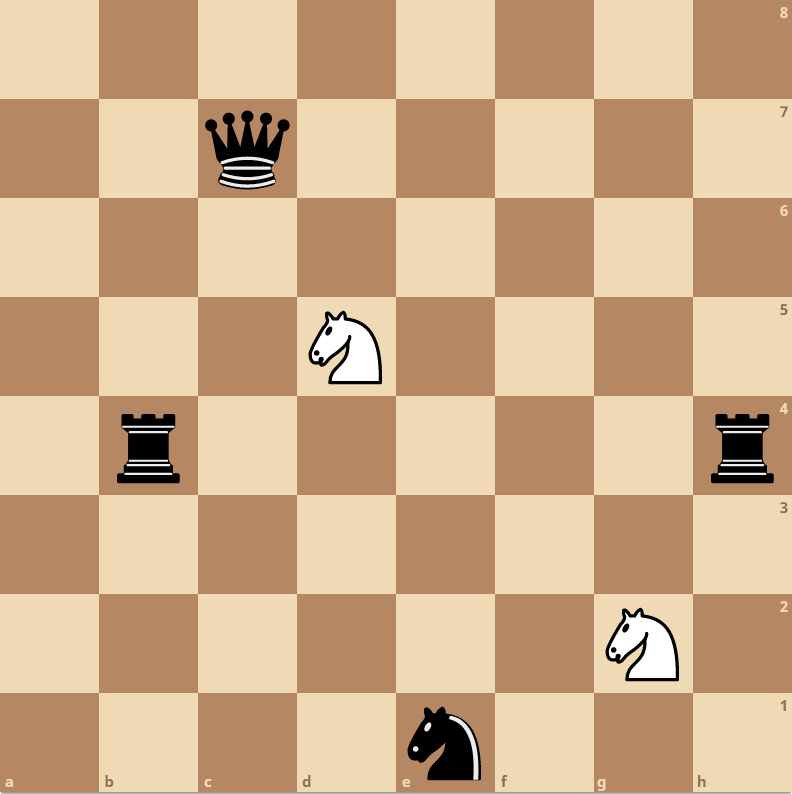
\includegraphics[width=170pt]{images/knightFork.png}
        \caption{Example of knight fork}
        \label{fig:knightFork}
    \end{subfigure}
    \caption{Examples of forks}
\end{figure}

\subsection{Connected Rooks}
\label{connectedRooks}
Er zijn 2 verschillende features, de \codeword{ConnectedRooksVertical()} en \codeword{ConnectedRooksHorizontal()} die op zo goed als hetzelfde werken. We gaan optellen hoeveel paren van torens er zijn die op ofwel dezelfde rang (horizontally connected) ofwel op dezelfde kolom staan (vertically connected) en waar geen andere stukken tussen staan.

\begin{figure}[h]
    \centering
    \begin{subfigure}{.4\textwidth}
        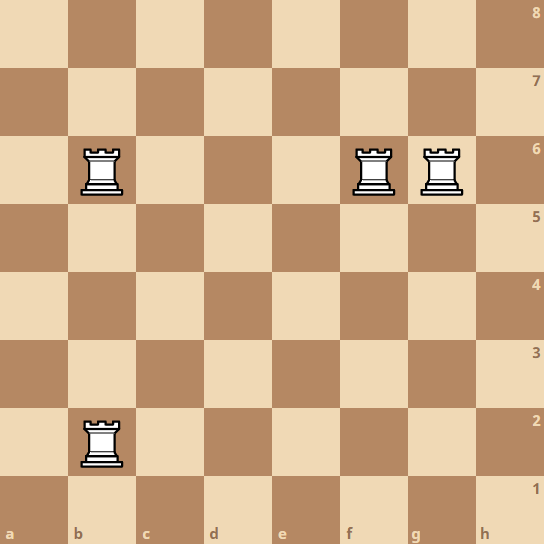
\includegraphics[width=170pt]{images/ConnectedRooks.png}
        \caption{Example of connected rooks}
        \label{fig:ConnectedRooks}
    \end{subfigure}
    \begin{subfigure}{.4\textwidth}
        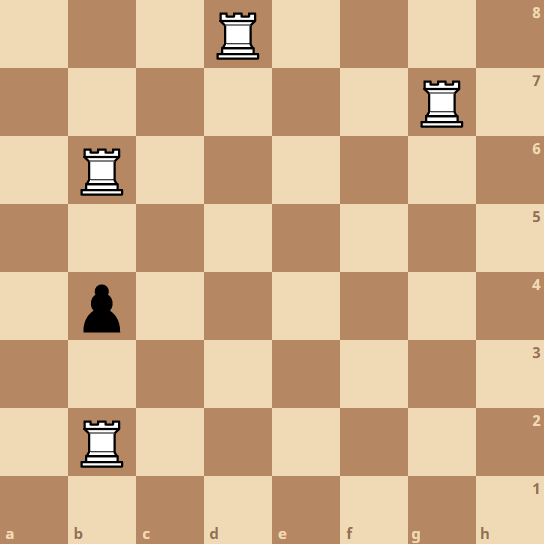
\includegraphics[width=170pt]{images/NotConnectedRooks.png}
        \caption{Example where rooks are not connected}
        \label{fig:NotConnectedRooks}
    \end{subfigure}
    \caption{Connected Rookd}
\end{figure}

In \figref{fig:ConnectedRooks} zien we op kolom b een vertically connected rooks en op rang 6 een horizontally connected rooks. Op \figref{fig:NotConnectedRooks} zijn er geen connected rooks omdat ze ofwel niet tegenover elkaar staan of er staat een stuk van de tegenspeler tussen.

\subsection{Control}
\subsubsection{Center Control}
Center control is een feature die ons verteld hoeveel pawn je hebt staan op de vakjes D4, E4, D5, E5. Deze 4 vakjes zijn het belangrijkste van het bord, omdat deze vakjes het grootste trafiek hebben van het bord.

Deze feature wordt ook weer voor zowel de eigen speler als de tegenspeler gecreëerd.

\subsubsection{Board Control}
Het aantal lege vakjes dat een speler met zijn stukken aanvalt, bepaald zijn controle over het bord. Deze feature bepaald dit aantal voor beide teams en trekt ze dan van elkaar af. Als meerdere stukken hetzelfde lege vakje kunnen aanvallen, wordt er rekening gehouden met de waarde van de stukken. Het kleinste stuk heeft dan het voordeel. Zo kan een toren kan dus nooit controle hebben over een vakje dat een pion van het andere ook kan aanvallen. 

\subsection{Connectivity}
\label{connectivity}

De connectivity beschrijft de mate waarin een speler zijn stukken kan beschermen. Met andere woorden: hoeveel ze geconnecteerd zijn met elkaar. Het kijkt dus niet enkel naar \reference{connectedRooks}, maar naar alle stukken die stukken van zijn eigen team kunnen 'aanvallen'. 

\subsection{Provokers}

Deze feature lijkt sterk op \reference{connectivity}. Het verschil zit erin dat we hier gaan kijken naar welke stukken we van de tegenspeler kunnen aanvallen. Ze dagen de stukken dus uit. 


\subsection{Position score}
We starten met het definiëren van een aantal matrices waarbij de matrix het bord voorstelt en elk vakje een bepaald score krijgt. Voor elk type schaakstuk hebben we een ingevulde matrix.

\begin{figure}[h]
    \centering
    \begin{subfigure}{.3\textwidth}
        $$
		\scalemath{0.6}{
		\begin{bmatrix}
		0& 0& 0& 0& 0& 0& 0& 0\\
		50& 50& 50& 50& 50& 50& 50& 50\\
		10& 10& 20& 30& 30& 20& 10& 10\\
		5& 5& 10& 25& 25& 10& 5& 5\\
		0& 0& 0& 20& 20& 0& 0& 0\\
		5& -5& -10& 0& 0& -10& -5& 5\\
		5& 10& 10& -20& -20& 10& 10& 5\\
		0& 0& 0& 0& 0& 0& 0& 0
		\end{bmatrix}}
		$$
        \caption{Pawn score matrix}

    \end{subfigure}
    \begin{subfigure}{.3\textwidth}
        $$
        \scalemath{0.6}{
		\begin{bmatrix}
		-50& -40& -30& -30& -30& -30& -40& -50\\
		-40& -20& 0& 0& 0& 0& -20& -40\\
		-30& 0& 10& 15& 15& 10& 0& -30\\
		-30& 5& 15& 20& 20& 15& 5& -30\\
		-30& 0& 15& 20& 20& 15& 0& -30\\
		-30& 5& 10& 15& 15& 10& 5& -30\\
		-40& -20& 0& 5& 5& 0& -20& -40\\
		-50& -40& -30& -30& -30& -30& -40& -50
		\end{bmatrix}}
		$$
        \caption{Knight score Matrix}
    \end{subfigure}
    \begin{subfigure}{.3\textwidth}
    	$$
    	\scalemath{0.6}{
    	\begin{bmatrix}
   		-20& -10& -10& -10& -10& -10& -10& -20\\
		-10& 0& 0& 0& 0& 0& 0& -10\\
		-10& 0& 5& 10& 10& 5& 0& -10\\
		-10& 5& 5& 10& 10& 5& 5& -10\\
		-10& 0& 10& 10& 10& 10& 0& -10\\
		-10& 10& 10& 10& 10& 10& 10& -10\\
		-10& 5& 0& 0& 0& 0& 5& -10\\
		-20& -10& -10& -10& -10& -10& -10& -20
		\end{bmatrix}}
		$$
		\caption{Bischop score matrix}
    \end{subfigure}
    \\
    \begin{subfigure}{.3\textwidth}
    	$$
    	\scalemath{0.6}{
    	\begin{bmatrix}
   		0& 0& 0& 0& 0& 0& 0& 0\\
		5& 10& 10& 10& 10& 10& 10& 5\\
		-5& 0& 0& 0& 0& 0& 0& -5\\
		-5& 0& 0& 0& 0& 0& 0& -5\\
		-5& 0& 0& 0& 0& 0& 0& -5\\
		-5& 0& 0& 0& 0& 0& 0& -5\\
		-5& 0& 0& 0& 0& 0& 0& -5\\
		0& 0& 0& 5& 5& 0& 0& 0
		\end{bmatrix}}
		$$
		\caption{Rook score matrix}
    \end{subfigure}
    \begin{subfigure}{.3\textwidth}
    	$$
    	\scalemath{0.6}{
    	\begin{bmatrix}
		-20& -10& -10& -5& -5& -10& -10& -20\\
		-10& 0& 0& 0& 0& 0& 0& -10\\
		-10& 0& 5& 5& 5& 5& 0& -10\\
		-5& 0& 5& 5& 5& 5& 0& -5\\
		0& 0& 5& 5& 5& 5& 0& -5\\
		-10& 5& 5& 5& 5& 5& 0& -10\\
		-10& 0& 5& 0& 0& 0& 0& -10\\
		-20& -10& -10& -5& -5& -10& -10& -20
		\end{bmatrix}}
		$$
		\caption{Queen score matrix}
    \end{subfigure}
    \begin{subfigure}{.3\textwidth}
    	$$
    	\scalemath{0.6}{
    	\begin{bmatrix}
		-30& -40& -40& -50& -50& -40& -40& -30\\
		-30& -40& -40& -50& -50& -40& -40& -30\\
		-30& -40& -40& -50& -50& -40& -40& -30\\
		-30& -40& -40& -50& -50& -40& -40& -30\\
		-20& -30& -30& -40& -40& -30& -30& -20\\
		-10& -20& -20& -20& -20& -20& -20& -10\\
		20& 20& 0& 0& 0& 0& 20& 20\\
		20& 30& 10& 0& 0& 10& 30& 20
		\end{bmatrix}}
		$$
		\caption{King score matrix}
    \end{subfigure}
    \caption{Score matrices}
\end{figure}

We gebruiken dit in de feature \codeword{PositionScoreBalance()} hierbij gaan we al onze schaakstukken af en sommeren we de punten van elk stuk met zijn overeenkomende plaats op de bijhorende matrix. Dit doen we voor zowel de speler als.

\subsection{Rooks on 7th rank}
Deze feature gaat kijken hoeveel torens er van de speler op de zevende rang staan. Hierbij wordt er geteld vanaf de kant van de speler zelf. Dus de tegenspeler zal dat dus rij 2 zijn. Wanneer er torens op de 7\ts{de} rang staat sta je heel sterk in het spel. Dit komt doordat je de bewegingsruimte van de opponent zijn koning sterk wordt beperkt en dat alle andere stukken op die rank niet veilig staan.

\begin{figure}[h]
    \centering
    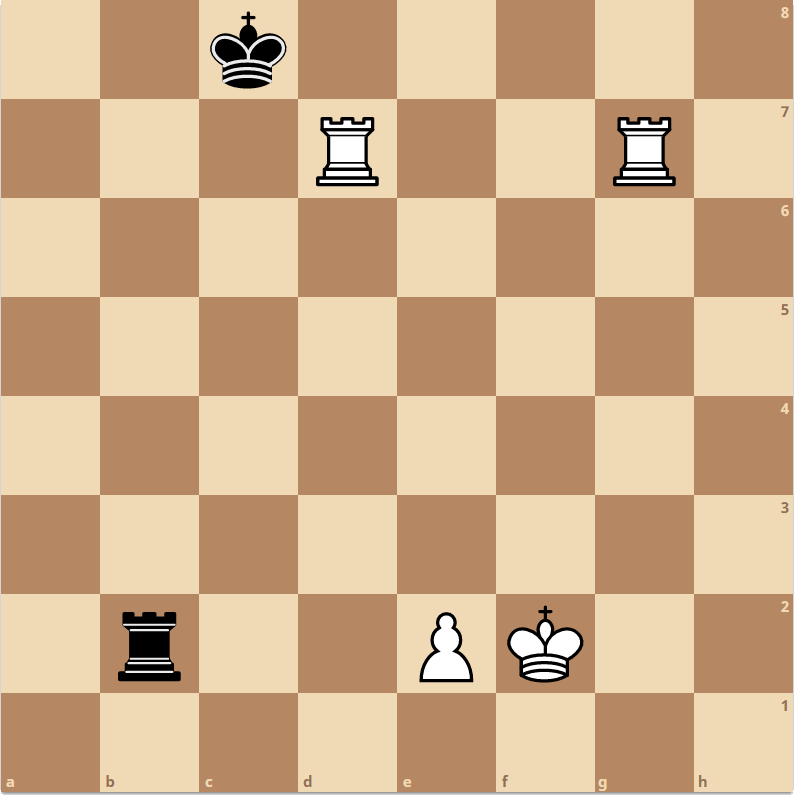
\includegraphics[width=170pt]{images/rooks7rank.png}
    \caption{Example of rooks on 7\ts{th} rank}
    \label{fig:rooks7rank}
\end{figure}


\subsection{King distance to center}
Zoals de naam het verteld zal deze feature de afstand van de koning tot één van de middelste vakjes berekenen. De middelste vakjes zijnde e4, d4, e5 en d5, we drukken de afstand uit in het aantal stappen dat de koning zou moeten nemen om in et midden terecht te komen.

\subsection{Castling}

Dit is een vrij eenvoudige feature die kijkt of de agent gecastled heeft. In \figref{fig:castling2} en \figref{fig:castling3} staan 2 voorbeelden afgebeeld van castling.

\begin{figure}[h]
    \centering
    \begin{subfigure}{.3\textwidth}
        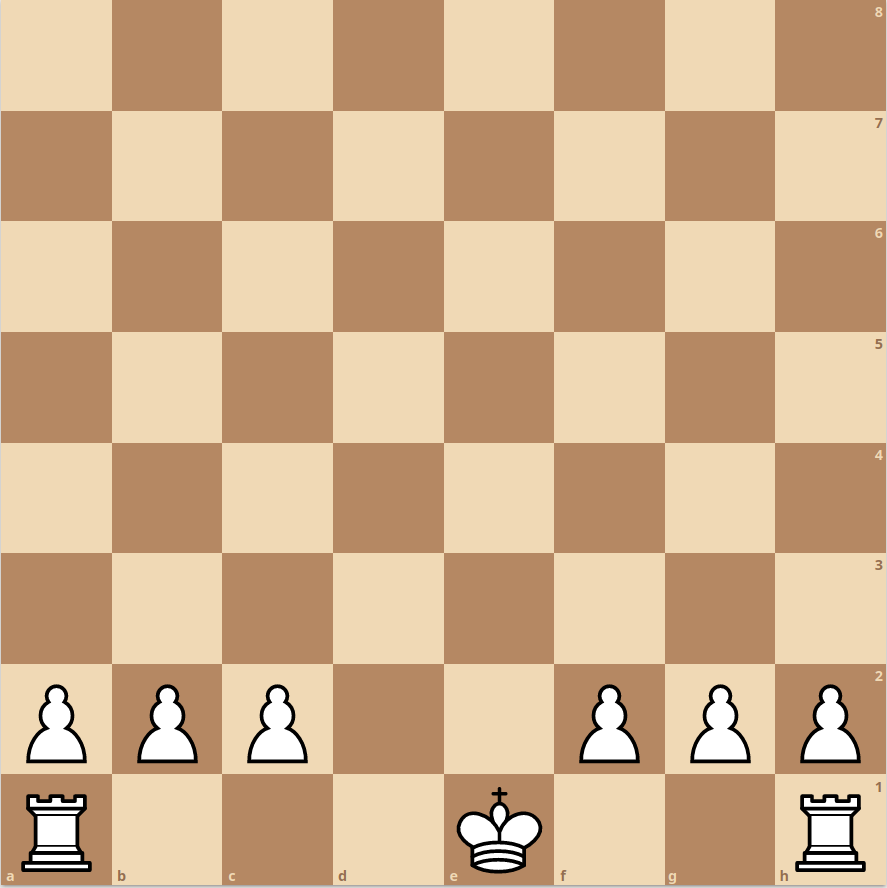
\includegraphics[width=130pt]{images/castling1.png}
        \caption{Initial state}
        \label{fig:castling1}
    \end{subfigure}
    \begin{subfigure}{.3\textwidth}
        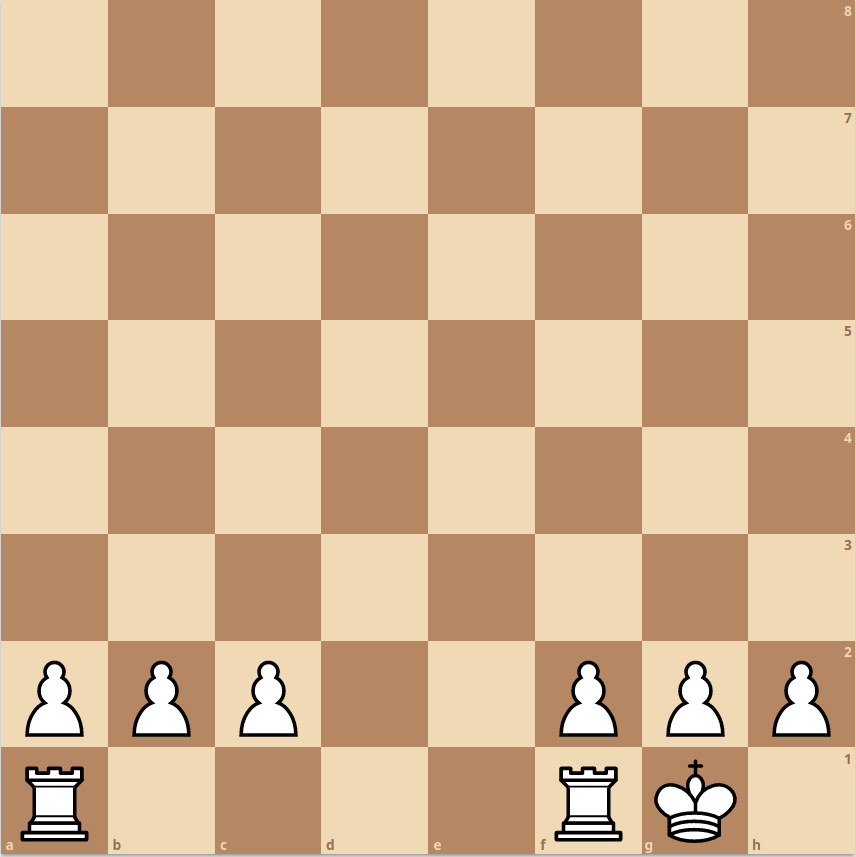
\includegraphics[width=130pt]{images/castling2.png}
        \caption{Short castling}
        \label{fig:castling2}
    \end{subfigure}
    \begin{subfigure}{.3\textwidth}
        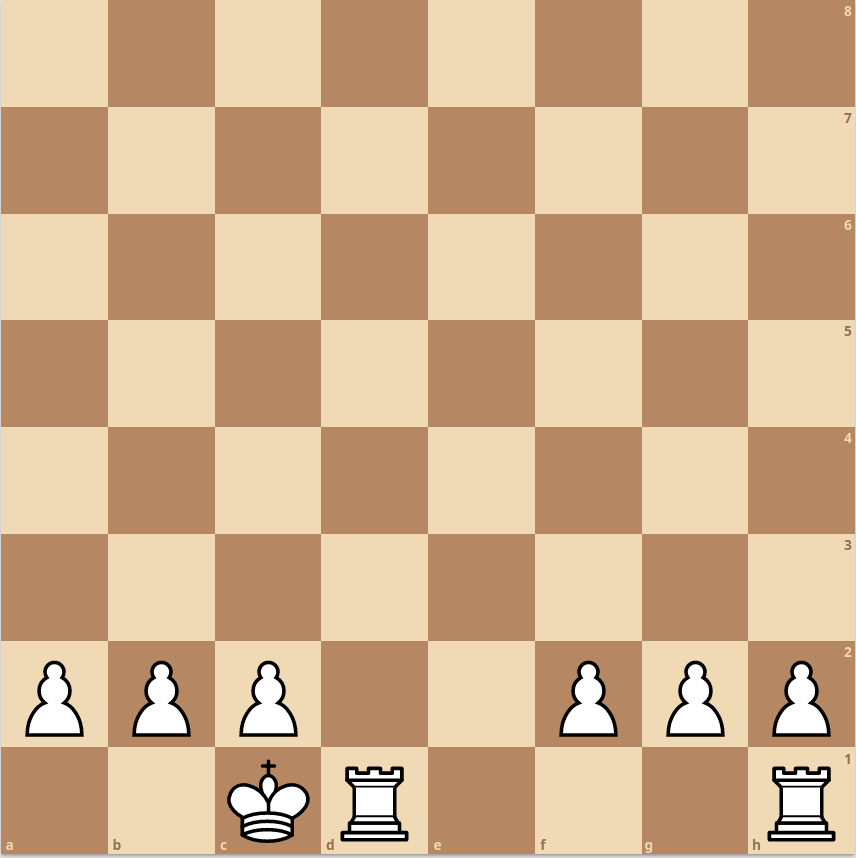
\includegraphics[width=130pt]{images/castling3.png}
        \caption{Long castling}
        \label{fig:castling3}
    \end{subfigure}
    \caption{Examples of castling}
    \label{fig:castling}
\end{figure}

\subsection{Light pieces on first rank}

Hier gaan we kijken of hoeveel van een speler zijn light pieces nog op de eerste rang staan. De eerste rang zal dus voor de speler rij 1 zijn en voor de tegenspeler rij 8. Met de light pieces verstaan we de paarden en lopers.

\begin{figure}[h]
    \centering
    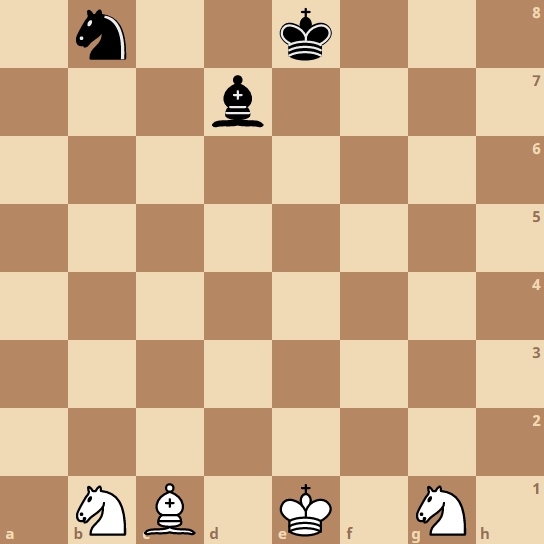
\includegraphics[width=170pt]{images/LightFirstRank.png}
    \caption{Example of Light pieces on 1\ts{th} rank}
    \label{fig:light1rank}
\end{figure}

In \figref{fig:light1rank} zal de witte speler een score van 3 krijgen voor zijn 2 paarden en loper. De zwarte speler heeft enkel een paard op zijn eerste rank staan en zal dus bij \codeword{LightFirstRankO()} een berekening van 1 krijgen.



\subsection{Doubled pawns}

Deze feature zal kijken hoeveel pionnen (meer als 1) er op één en dezelfde lijn staan (mag zowel horizontaal als verticaal).


\subsection{Alpha-beta Agent prediction feature}

Deze feature laat een onze alpha-beta agent een keuze maken in de huidige situatie. Als deze keuze overeenkomt met de keuze van de Q-agent dan returned deze feature $1$ zo niet dan krijgen we een return waarde van $0$. Deze feature kent ook optimalisaties maar hierover later meer in \reference{caching}.




\section{Reward}

De reward functie is als volgt gedefinieerd:


$$
R(S, a, NS) = 
\begin{cases}
    100 &\mbox{Schaakmat gewonnen}\\
    -30 &\mbox{Gelijkspel of Stalemate}\\
    -100 &\mbox{Schaakmat verloren}\\
     C_O(S, a) - C_S(NS) + c(S) + \Delta M &\mbox{Bij overige situaties}
\end{cases}
$$

\begin{conditions}
    C_O & of de opponent in schaak staat\\
    C_S & of de agent in schaak staat\\
    c &   of er gecastled is\\
    \Delta M & het materiaal verschil op het bord
\end{conditions}


\chapter{Optimalisaties}

We hebben een hoop optimalisaties moeten toevoegen aan onze Q-Learner om hem zo rap mogelijk te laten denken.

\section{Multi-Threading}

We hebben multi-threading toegevoegd aan onze q-learner zo berekent hij de q-waarde van elke actie in een aparte thread. We hebben bewust niet gekozen om elke feature apart omdat dit onze timing issues verergerde in plaat van verbeterde. We hebben door multi-threading onze iteratie tijd met $20\%$ weten dalen.

In \figref{fig:singlethreaded} en \figref{fig:multithreaded} is het verschil te zien tussen single-threaded \tiny(\ref{fig:singlethreaded})\small{ }en multi-threaded \tiny(\ref{fig:multithreaded})\small{ }CPU usage.

\begin{figure}[h]
    \centering
    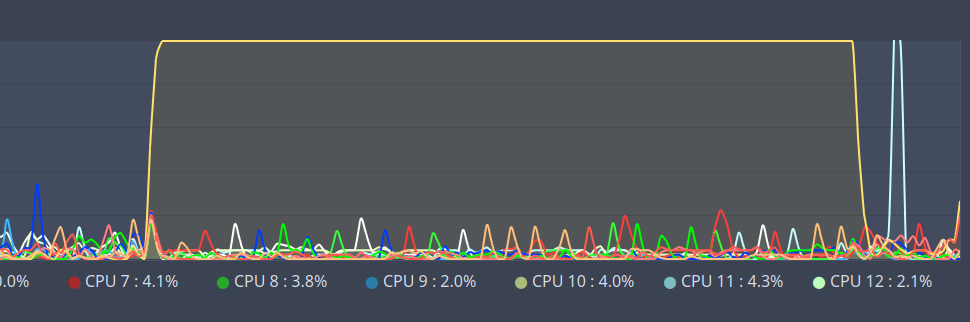
\includegraphics[width=300pt]{images/singlethreaded.png}
    \caption{Single Threaded Q-Learner CPU usage}
    \label{fig:singlethreaded}
\end{figure}

\begin{figure}[h]
    \centering
    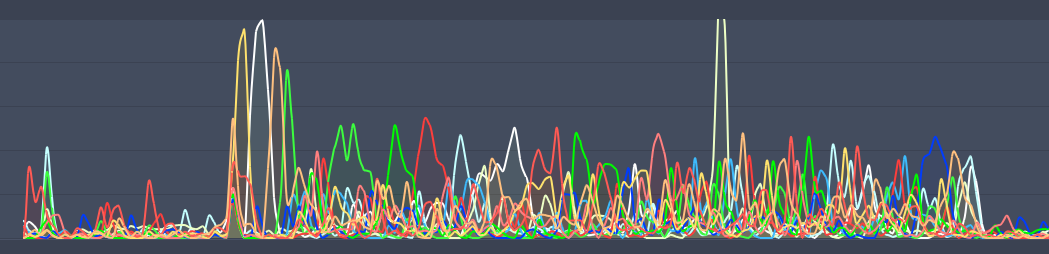
\includegraphics[width=350pt]{images/multithreaded.png}
    \caption{Multi Threaded Q-Learner CPU usage}
    \label{fig:multithreaded}
\end{figure}

\section{Caching}
\label{caching}

We gebruiken ook veel plaatsen caching zodat we niet 2 keer hetzelfde moeten uitrekenen. De meest bijzondere cache is deze voor onze alpha-beta feature, deze moet per bord state maar 1 keer uitvoeren waardoor we de alpha-beta langer kunnen laten zoeken en een hoop tijd besparen.
De tijd die we hierdoor besparen per iteratie kan soms tot een minuut of 2 oplopen.

Dit was uiteraard wel een trade off met memory usage, echter werd de extra gebruikte memory overschaduwd door de tijdswinsten.

\chapter{Resultaten}

Hier vind je al onze resultaten van het uitbundig trainen. We hebben deze in de loop van 5 dagen op een cloud server laten trainen. 1 dag tegen stockfish en de overige 4 dagen tegen onze alpha-beta agent.

Je kan ook altijd onderaan de commando's vinden die we gebruikt hebben bij het trainen van onze agent.

\section{GrandQ vs. Stockfish}

In de eerste leer sessie hebben we onze Q-agent tegen stockfish laten trainen zoals verwacht heeft onze agent nooit kunnen winnen, maar heeft wel hieruit nuttige info kunnen leren.

Command:\\
\codeword{python3 train -o stockfish --skill 0 --depth 3 -tt 15 -dt 0 -e 0.3 -d 0.3 -l 0.01 -q -i -1}

\begin{figure}[h]
    \centering
    \begin{subfigure}{.45\textwidth}
        \centering
        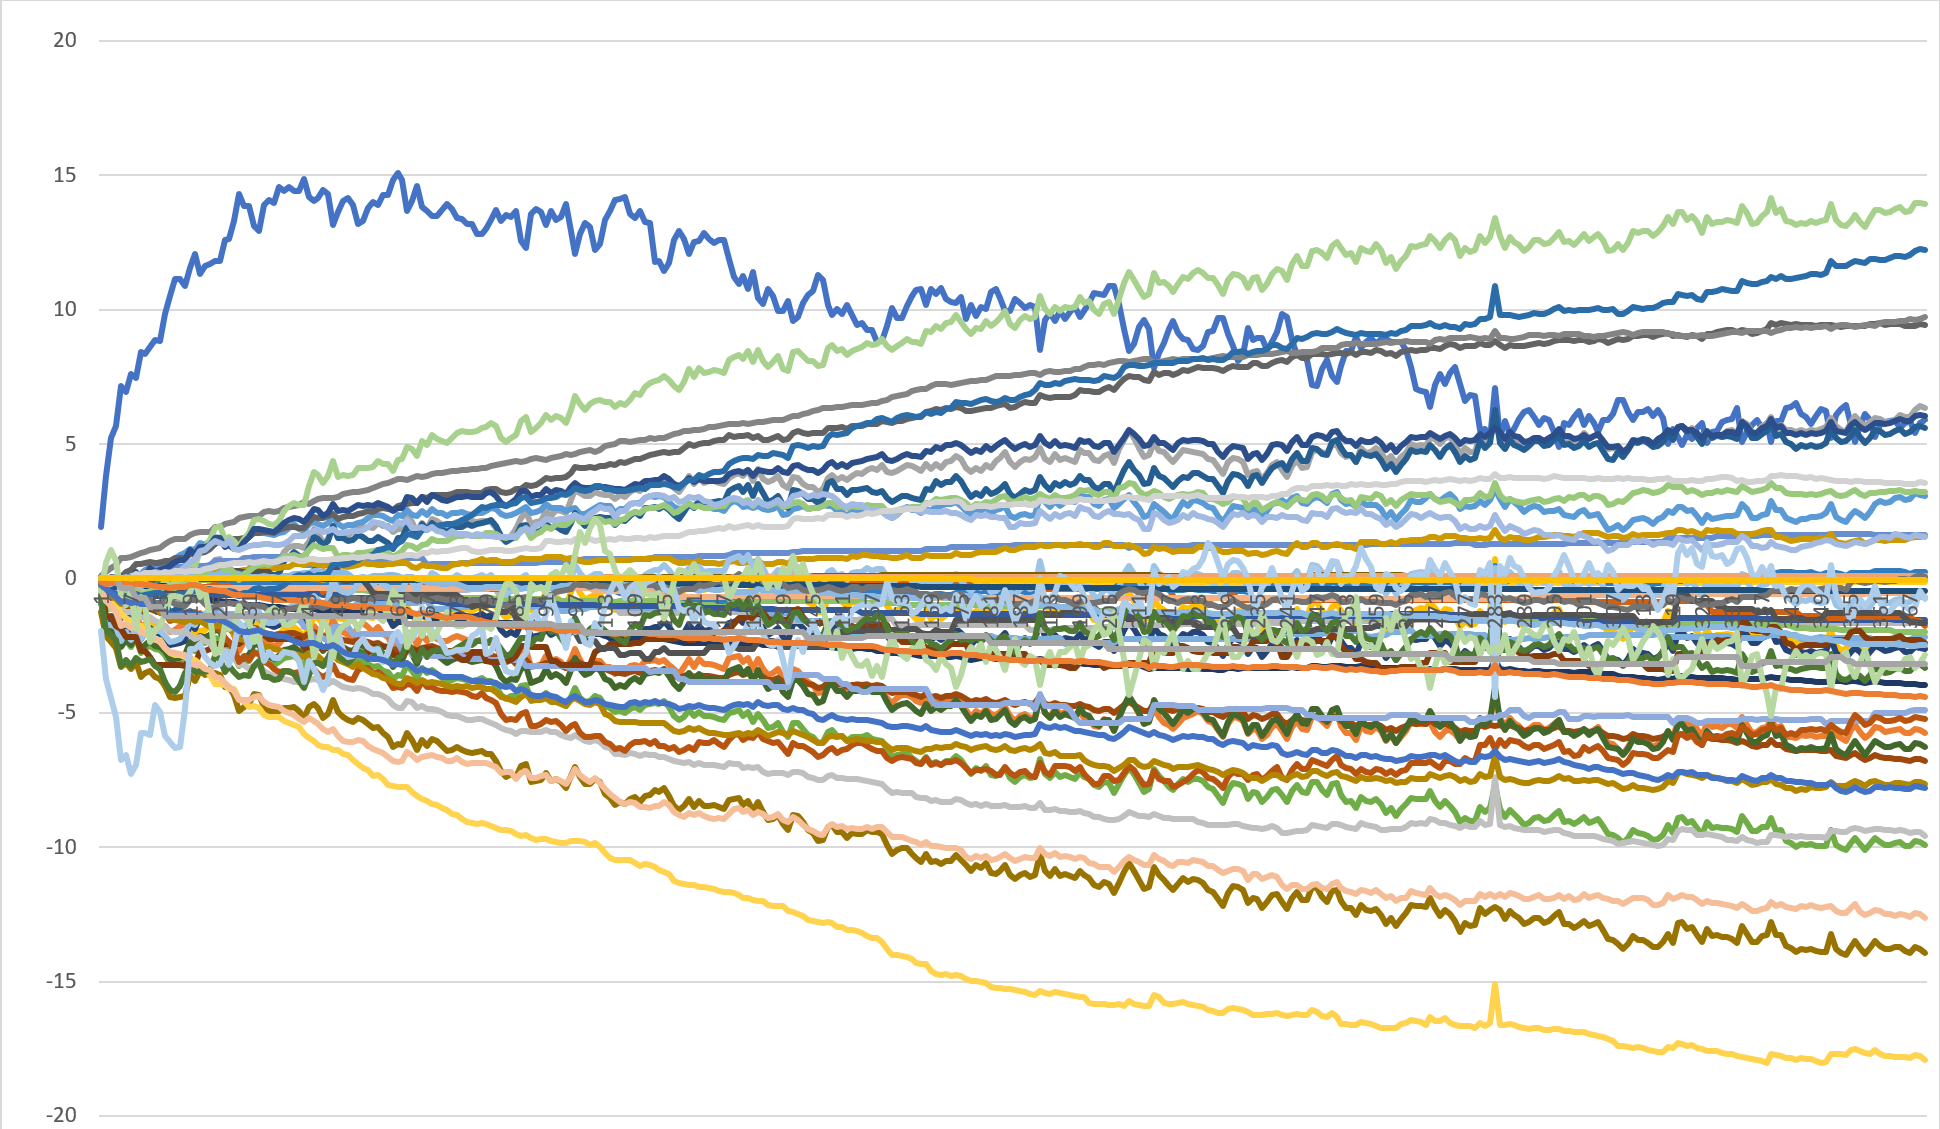
\includegraphics[width=\textwidth]{images/EXCEL_2020-12-12_18-01-58.png}
        \caption{All features except checkmates}
    \end{subfigure}
    \begin{subfigure}{.45\textwidth}
        \centering
        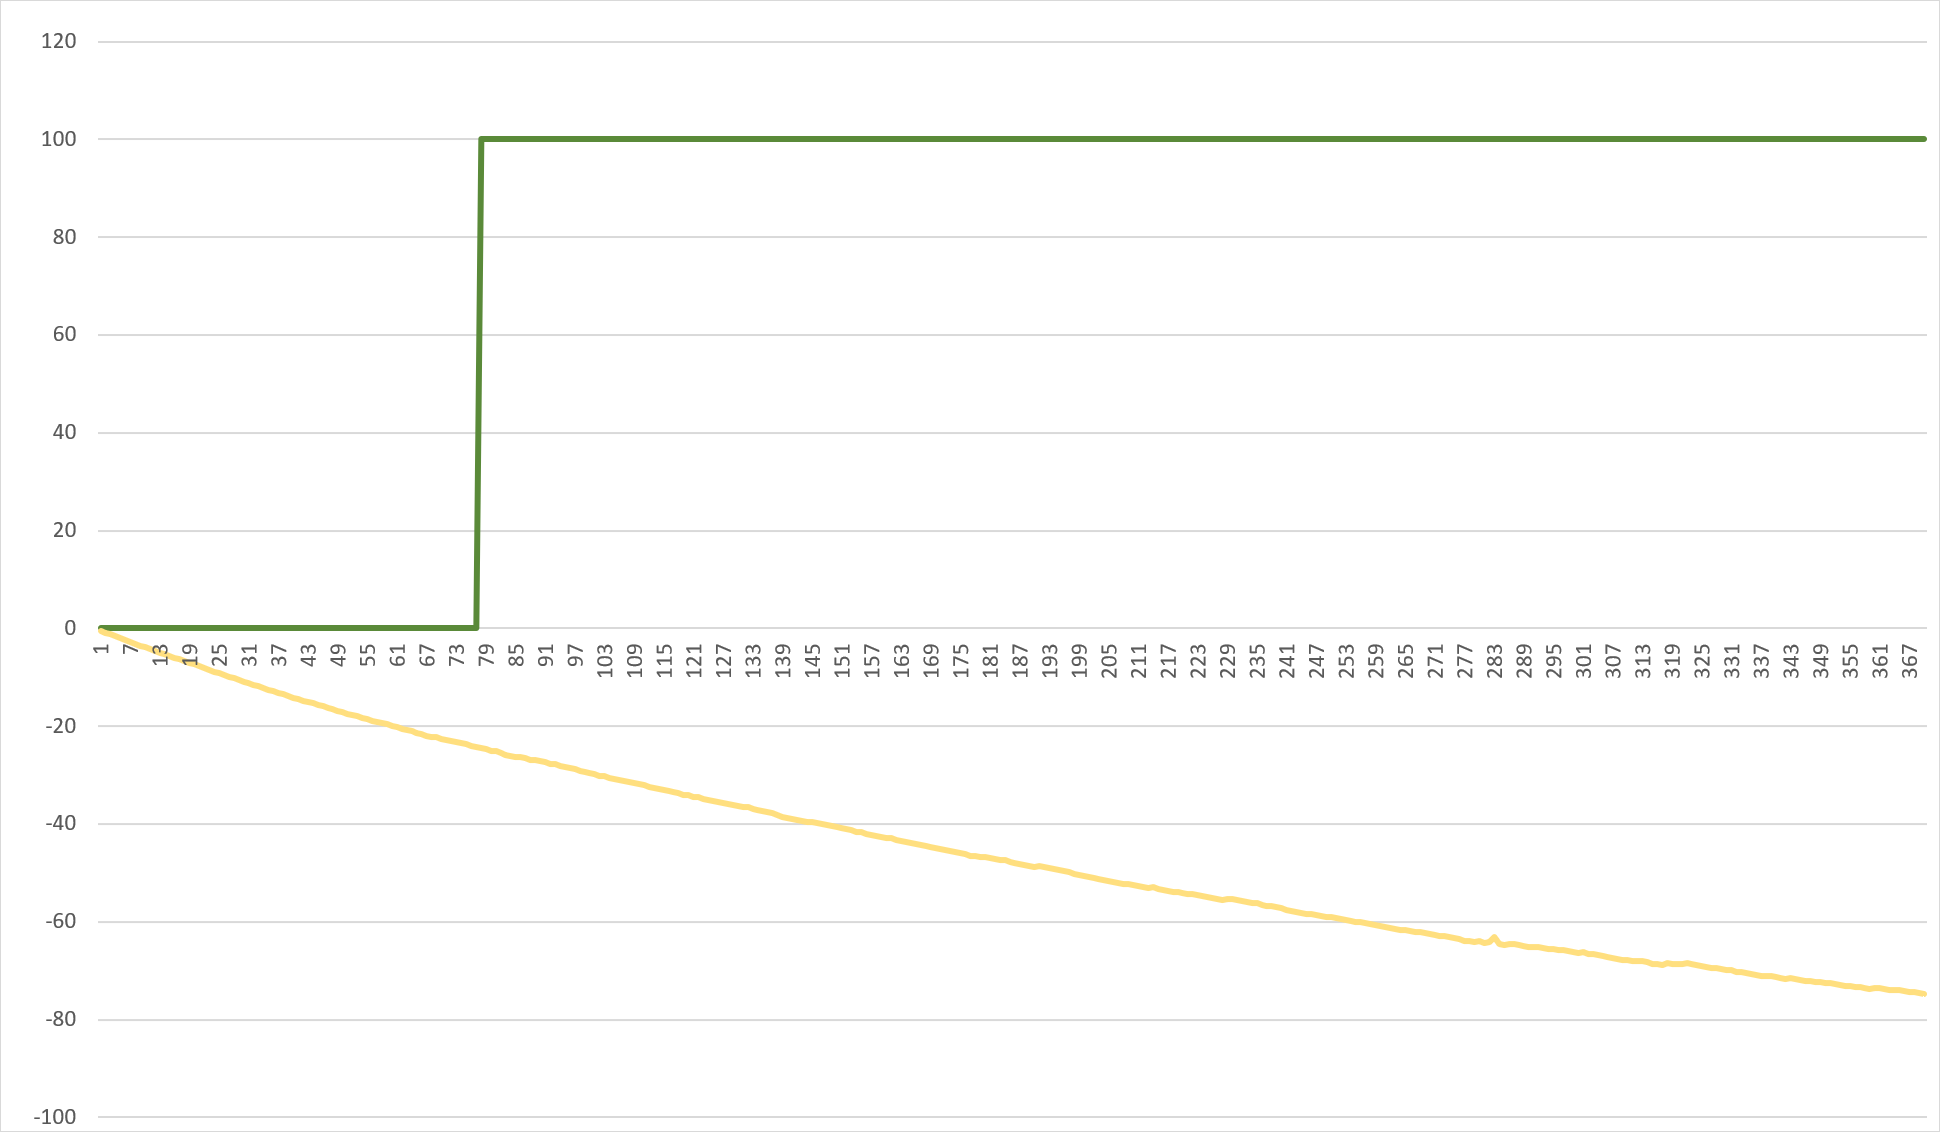
\includegraphics[width=\textwidth]{images/EXCEL_2020-12-12_18-01-10.png}
        \caption{Check mate \& Next Checkmate}
    \end{subfigure}
    \caption{Weight history vs. Stockfish}
\end{figure}

\pagebreak

\section{GrandQ vs. Alpha-Beta}

Later hebben we nog een paar spelletjes gespeeld tegen onze alpha-beta agent. Deze waren bijna allemaal gewonnen.

Command:\\
\codeword{python3 train -o ab --depth 3 -tt 15 -dt 0 -e 0.3 -d 0.3 -l 0.01 -q -i -1}

\begin{figure}[h]
    \centering
    \begin{subfigure}{.45\textwidth}
        \centering
        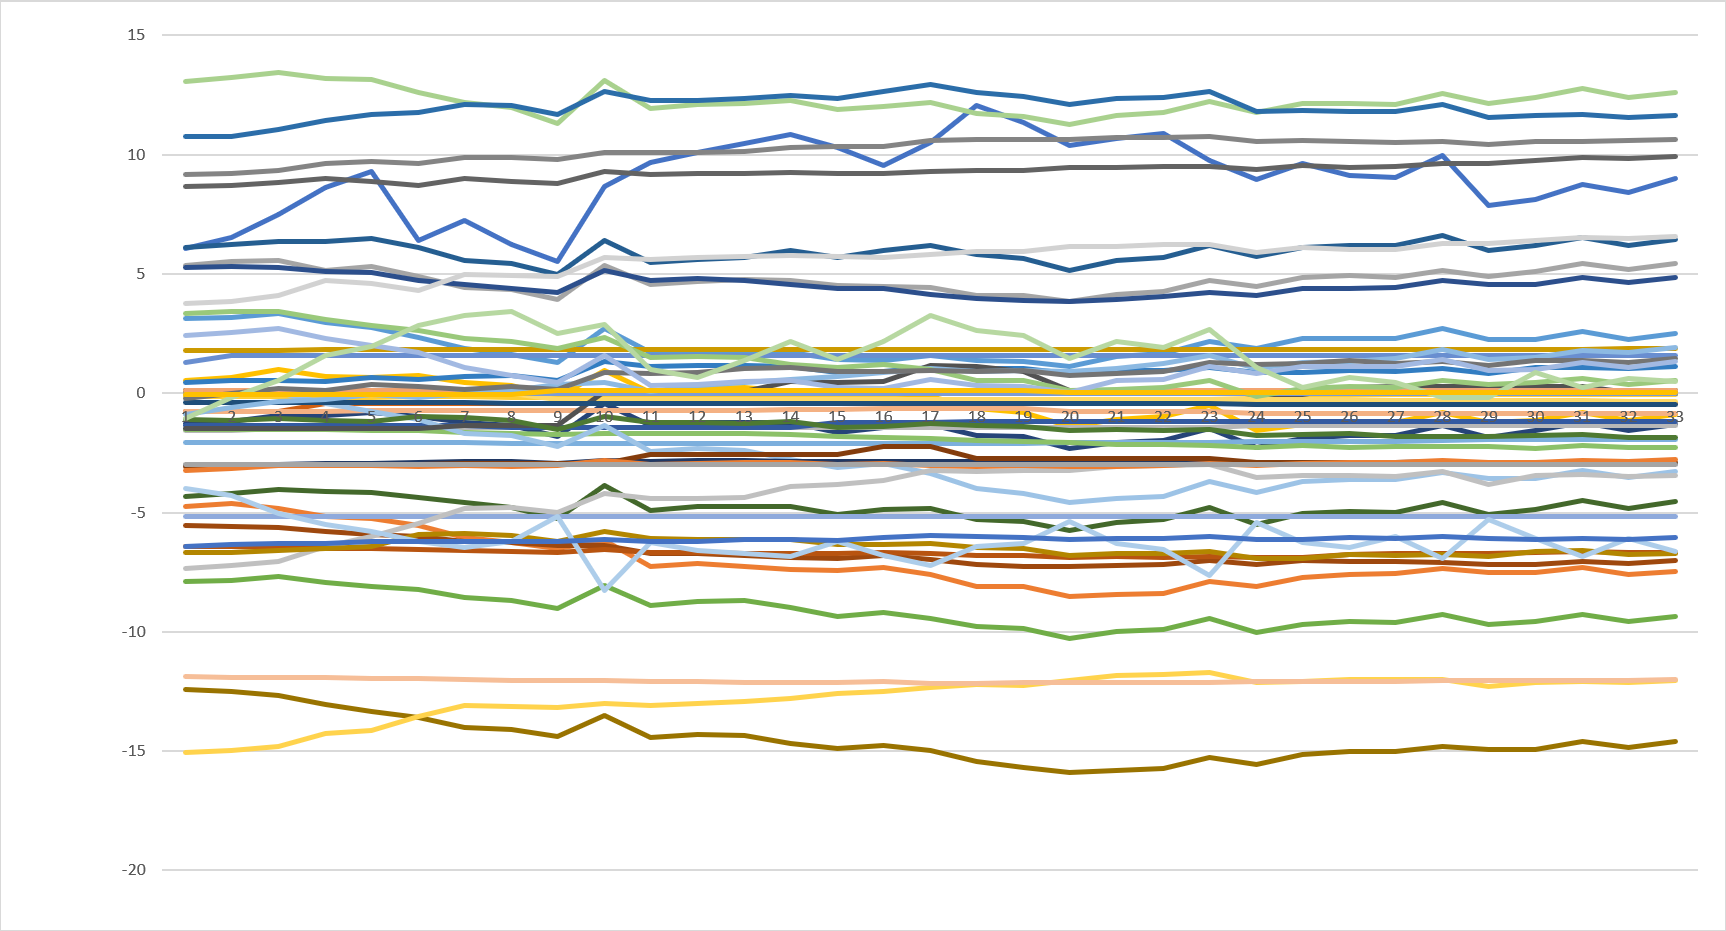
\includegraphics[width=\textwidth]{images/EXCEL_2020-12-12_18-02-40.png}
        \caption{Weight history vs. Stockfish}
        \label{fig:ab}
    \end{subfigure}
    \begin{subfigure}{.45\textwidth}
        \centering
        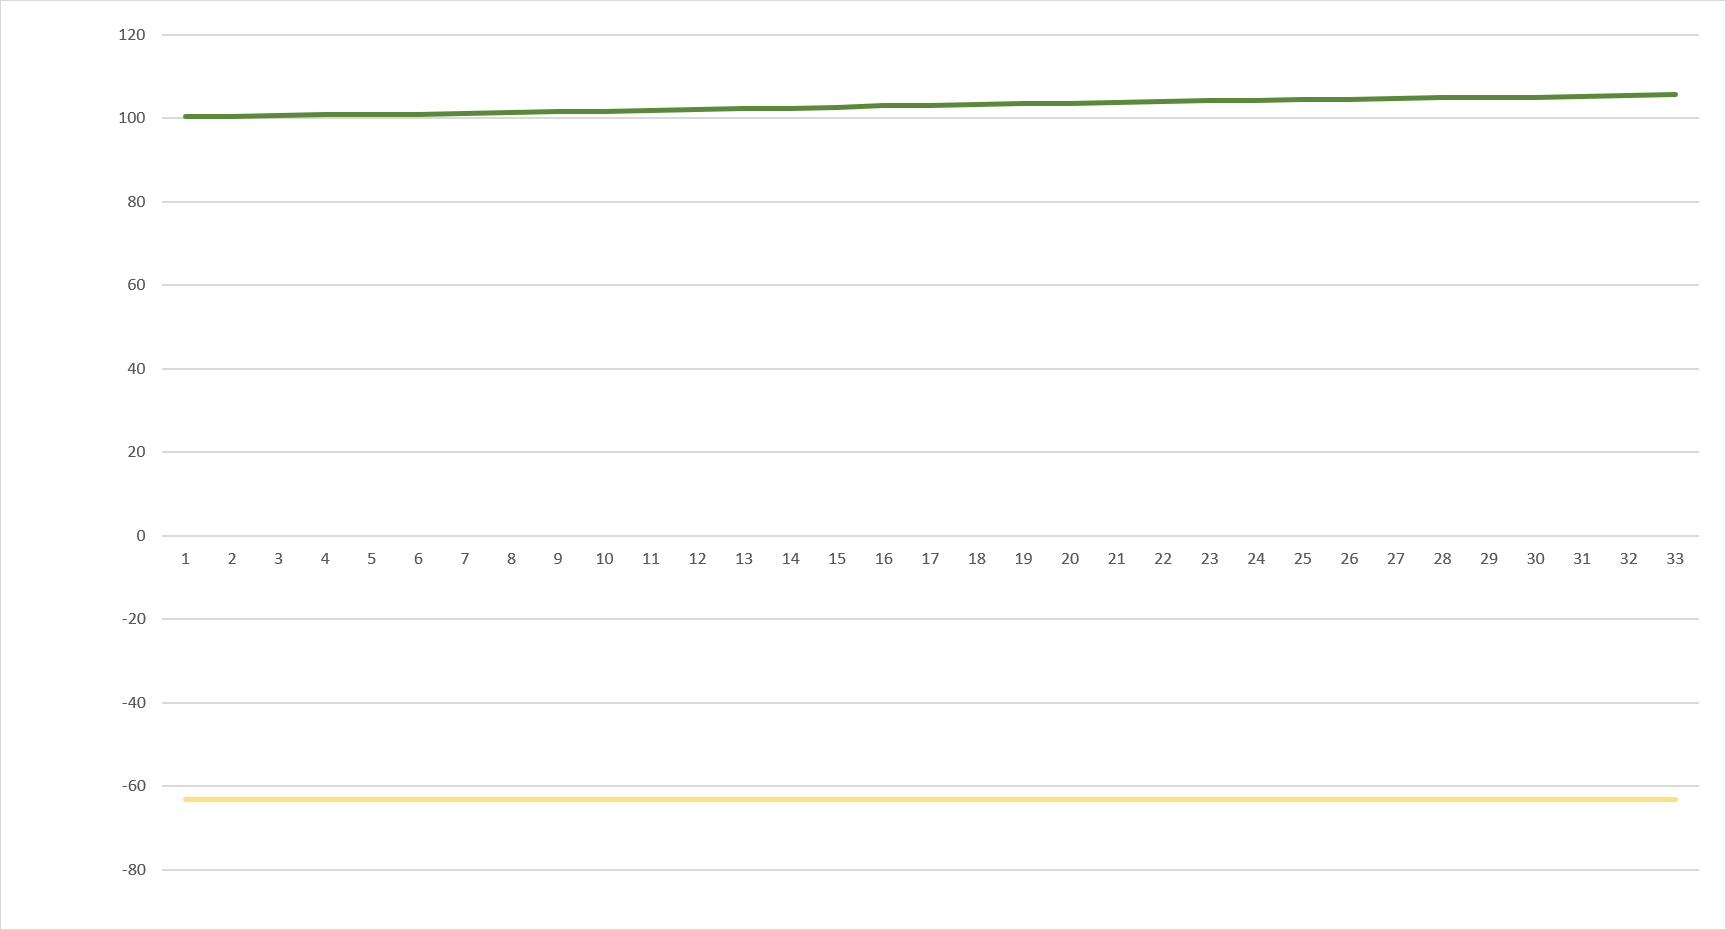
\includegraphics[width=\textwidth]{images/EXCEL_2020-12-12_17-58-38.png}
        \caption{Check mate \& Next Checkmate}
        \label{fig:abc}
    \end{subfigure}
    \caption{Weight History vs. Alpha-Beta}
\end{figure}

\section{Git Repository:}
Onze code en ons getrained bestand is ook terug te vinden op gitlab: 
\begin{itemize}
    \item Repository: \href{https://gitlab.com/Artificiele_Intelligentie/chess}{\color{blue}\underline{https://gitlab.com/Artificiele\_Intelligentie/chess}}
    \item \href{https://gitlab.com/Artificiele_Intelligentie/chess/-/raw/master/grandQ.json}{\color{blue}\underline{Getraind bestand}}
\end{itemize}

\bibliography{sources}
\bibliographystyle{ieeetr}

\end{document}
